\documentclass[11pt,a4paper]{report}
\usepackage[utf8]{inputenc}
\usepackage[french]{babel}
\usepackage[T1]{fontenc}
\usepackage{amsmath}
\usepackage{amsfonts}
\usepackage{amssymb}
\usepackage{graphicx}
\usepackage[left=2cm,right=2cm,top=2cm,bottom=2cm]{geometry}
\usepackage{commath}  % pour les dérivées partielles/ordinaires : \od et \pd

\title{Correction examen première session 2016-2017}
\author{Loan Sens\\ en collaboration avec\\Robin Petit}

\newcommand{\rac}{\ensuremath{\frac{\sqrt{2}}{2}}}

\DeclareMathOperator{\Jac}{Jac}

\begin{document}
	\maketitle

	Je ne garantis en rien l'exactitude de chacune des réponses qui va suivre, ce corrigé est surtout pour donner une idée générale pour comprendre comment réussir les examens de INOFO-F-305. ;)

	\section*{Question 1}
		Considérons le système non linéaire continu suivant :
		\[
		\begin{cases}
			\dot{x_1} = x_1^2 + x_2^2 -1 \\
			\dot{x_2} = x_1^2 - x_2^2
		\end{cases}
		\]
		où $x_1 \in [-5, 5]$ et $x_2 \in [-5, 5]$.

		L'étudiant devra~:
		\begin{enumerate}
			\item calculer analytiquement le(s) point(s) d'équilibre~;
			\item étudier la stabilité du(des) point(s) d'équilibre (du système non-linéaire) par linéarisation~;
			\item tracer sur du papier millimétré le portrait de phase avec les isoclines du systèmes \& comportement qualitatif des trajectoires autour du(des) point(s) d'équilibre \& le comportement
			qualitatif des 4 trajectoires dont les points initiaux sont : $(0,0) , (1,1), (-1, -2), (-2,0)$.
		\end{enumerate}
		\pagebreak

		\subsection*{1) calculer analytiquement le(s) point(s) d'équilibre}
			Pour cela nous analyserons les isoclines du système.

			Soit~:
			\[
			\begin{cases}
				I_1 \equiv \dot{x_1} = 0 \\
				I_2 \equiv \dot{x_2} = 0.
			\end{cases}
			\]

			En développant~:
			\[
			\begin{cases}
				I_1 \equiv x_1^2 + x_2^2 = 1 \\
				I_2 \equiv x_1^2 = x_2^2
			\end{cases}
			\]

			La première équation est celle d'un cercle dont le centre est l'origine du repère de rayon 1. La seconde est celle de 2 droites de pentes 1 et -1 se croisant en l'origine, désignant donc
			les deux segments de droites définis par $x_1 = \pm x_2$ sur $[-5, 5] \times [-5, 5]$.

			Il y a 4 points d'intersection entre les 2 isoclines qui seront nos points d'équilibres~:
			\[
				I_1 \cap I_2 = \left\{\left( \rac , \rac\right), \left( -\rac , \rac\right), \left(\rac , -\rac\right), \left(-\rac , -\rac\right)\right\}.
			\]

		\subsection*{2) étudier la stabilité du(des) point(s) d'équilibre (du système non linéaire) par linéarisation}

			Pour cela nous avons besoin de la Jacobienne du champ de vecteurs du système~:
			\[
				(\Jac f)(x_1, x_2)
				=
				\begin{bmatrix}
			   	\pd {f_1}{x_1}(x_1, x_2) & \pd {f_1}{x_2}(x_1, x_2) \\
			   	\pd {f_2}{x_1}(x_1, x_2) & \pd {f_2}{x_2}(x_1, x_2)
				\end{bmatrix}
				=
				\begin{bmatrix}
			   	2x_1 & 2x_2 \\
			   	2x_1 & -2x_2
				\end{bmatrix}
			\]

			Pour~:
			\begin{itemize}
				\item $(x_1, x_2) = \left(\rac , \rac\right)$~:
					\[\det\left((\Jac f)(x_1, x_2) - \lambda I\right) = \det
					\begin{bmatrix}
			   		2 \cdot \rac - \lambda & 2\cdot \rac \\
			   		2\cdot \rac & -2\cdot \rac  - \lambda
					\end{bmatrix}= 0,
					\]
					donc~:
					\[
						((\sqrt{2} - \lambda) \cdot (- \sqrt{2} - \lambda)) - (\sqrt{2} \cdot \sqrt{2}) = 0 \Leftrightarrow \lambda^2 - 4 = 0.
					\]
					Les solutions de ce système sont $\lambda_{1,2} = \pm 2$. Étant donné que nous avons 2 racines réelles de signe opposé, l'état d'équilibre est une \emph{selle} dans le système
					linéarisé (et donc dans le système initial également), on déduit que cet état d'équilibre est instable.

				\item $(-\rac , \rac)$~:

					Même raisonnement...
					\begin{gather*}
						\lambda^2 + 2\sqrt{2}\cdot\lambda+4 = 0	\\
						\Delta = -8 \\
						\lambda_{1,2} = -\sqrt{2} \pm i\sqrt{2}
					\end{gather*}
					Étant donné que les valeurs propres sont complexes conjuguées de partie réelle non-nulle, et négatives, on déduit que l'état d'équilibre est un foyer \textit{stable} dans le système
					linéarisé, et donc de même pour le système initial.

				\item $(\rac , -\rac)$ : \\
					Même raisonnement...
					\begin{gather*}
						\lambda^2 - 2\sqrt{2}\cdot\lambda+4 = 0	\\
						\Delta = -8 \\
						\lambda_{1,2} = \sqrt{2} \pm i\sqrt{2}
					\end{gather*}
					Idem, si ce n'est partie réelle positive donc foyer \textit{instable} (donc toujours valide pour le système initial).

				\item $( -\rac , -\rac)$ : \\
					Même raisonnement...
					\begin{gather*}
						\lambda^2 - 4 = 0
					\end{gather*}
					On trouve le même système qu'au premier point et donc là aussi nous avons une \emph{selle}, et donc un point d'équilibre instable.
			\end{itemize}

		\subsection*{3) tracer sur du papier millimétré le portrait de phase avec les isoclines du systèmes \& comportement qualitatif des trajectoires autour du(des) point(s) d'équilibre \& le comportement
		qualitatif des 4 trajectoires dont les points initiaux sont : $(0,0) , (1,1), (-1, -2), (-2,0)$}

			Voir schéma ci-dessous (dessiné par Liran).

			Pour les trajectoires~:
			\begin{itemize}
				\item $(0,0)$~:
					\[
					\begin{cases}
						\dot{x_1} = 0^2 + 0^2 -1 \\
						\dot{x_2} = 0^2 - 0^2
					\end{cases}
					= (-1,0).
					\]
					Remarquons que c'est normal que $\dot {x_2} = 0$ car $(0,0) \in I2$.

				\item $(1,1)$~:
					\[
					\begin{cases}
						\dot{x_1} = 1^2 + 1^2 -1 \\
						\dot{x_2} = 1^2 - 1^2
					\end{cases}
					= (1,0).
					\]

				\item $(-1,-2)$~:
					\[
					\begin{cases}
						\dot{x_1} = (-1)^2 + (-2)^2 -1 \\
						\dot{x_2} = (-1)^2 - (-2)^2
					\end{cases}
					= (4, -3).
					\]

				\item $(-2,0)$~:
					\[
					\begin{cases}
						\dot{x_1} = (-2)^2 + 0^2 -1 \\
						\dot{x_2} = (-2)^2 - 0^2
					\end{cases}
					= (3, 4).
					\]
			\end{itemize}

			\includegraphics[width=\textwidth]{"portrait-de-phase"}
			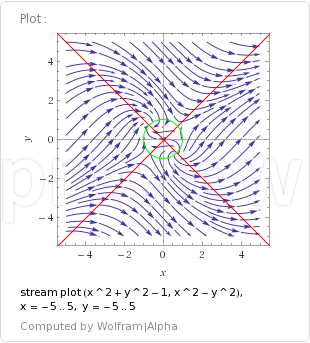
\includegraphics[width=\textwidth]{portrait-de-phase_wolfram}




	\pagebreak
	\section*{Question 2}
		Considérons le système à temps discret décrit par l'équation suivante :
		\[
			E \equiv a \cdot x(k+2) + x(k) = k^2 + k + 1 \qquad a \in \mathbb{R} \setminus \{0, -1\}.
		\]

		\begin{enumerate}
			\item Donnez la solution générale de l'équation homogène~;
			\item Donnez la solution particulière de l'équation de départ~;
			\item Donnez la solution générale de l'équation non-homogène sachant que~: $a=3,\ x(0) = 0,\ x(1) = 1$~;
			\item Sachant que~: $a=3,\ x(0) = 0,\ x(1) = 1$, calculez la valeur de $x(k)$ pour $k \in \{ 0,1,2,3,4 \}$.
		\end{enumerate}
		\pagebreak

		\subsection*{1) Donnez la solution générale de l'équation homogène}
		L'équation homogène de ce système est donné par :
		\[
			EH \equiv a \cdot x^2 + 1 = 0
		\]
		Trouvons les racines de cette équation en fonctions des valeurs de $a$ :
		\[
			\Delta = -4a
		\]
		\begin{itemize}
			\item $\Delta = 0 \Leftrightarrow -4a = 0 \Leftrightarrow a = 0$ or $a \neq 0$, donc $\Delta$ ne peut pas valoir $0$.
			\item $\Delta > 0 \Leftrightarrow -4a > 0 \Leftrightarrow a < 0$\\
				\[
					\lambda_{1,2} = \frac{-b \pm \sqrt{\Delta}}{2a} = \pm \frac{\sqrt{-a}}{a}
				\]
				$a < 0$ donc pas de soucis de racine négative.
				\[
					SG_{a<0} \equiv  x^{(G)}(k) = c_1 \left(\frac{\sqrt{-a}}{a} \right)^k + c_2\left(-\frac{\sqrt{-a}}{a}\right)^k
				\]

			\item $\Delta > 0 \Leftrightarrow -4a > 0 \Leftrightarrow a > 0$\\
				\[
					\lambda_{1,2} = \frac{-b \pm i\sqrt{\Delta}}{2a} = \pm i\frac{\sqrt{a}}{a} \rightarrow \alpha = 0 \quad \beta = \frac{\sqrt{a}}{a}
				\]
				$a > 0$ donc pas de soucis de racine négative.
				\begin{gather*}
					\rho = \sqrt{\alpha^2 + \beta^2} = \frac{\sqrt{a}}{a} \\
					\begin{cases}
						\cos(\theta) = \frac{\alpha}{\rho} = 0\\
						\sin(\theta) = \frac{\beta}{\rho} = 1
					\end{cases}
					\Leftrightarrow \theta = \pi/2,
				\end{gather*}
				ou plus simplement, la solution est imaginaire pure donc sous la forme $\beta i = \rho\exp(i\theta)$, avec donc $\rho = \beta$ et $\theta = \frac \pi2$.
				\[
					SG_{a>0} \equiv  x^{(G)}(k) = c_1 \left(\frac{\sqrt{a}}{a} \right)^k \cos\left(k \frac{\pi}{2}\right) + c_2\left(\frac{\sqrt{a}}{a}\right)^k \sin\left(k \frac{\pi}{2}\right)
				\]
		\end{itemize}

		\subsection*{2) Donnez la solution particulière de l'équation de départ}
			Nous devons donc trouver une fonction $x^{(P)}(k)$ telle que $a \cdot x^{(P)}(k+2) + x^{(P)}(k) = k^2 + k + 1$. Cherchons donc la solution sous forme d'équation du second degré
			(comme le membre de droite). Posons~:
			\[
				x^{(P)}(k) = \alpha_1 \cdot k^2 + \alpha_2 \cdot k + \alpha_3
			\]
			et donc :
			\begin{align*}
				x^{(P)}(k+2) &= \alpha_1 \cdot (k+2)^2 + \alpha_2 \cdot (k+2) + \alpha_3 \\
					&= \alpha_1 k^2 + 4\alpha_1k + 4\alpha_1 + \alpha_2 k + 2\alpha_2 + \alpha_3
			\end{align*}

			Injectons dans l'équation de départ :
			\begin{gather*}
				a \cdot x^{(P)}(k+2) + x^{(P)}(k) = k^2 + k + 1\\
				a \cdot (\alpha_1 k^2 + 4\alpha_1k + 4\alpha_1 + \alpha_2 k + 2\alpha_2 + \alpha_3) + (\alpha_1 \cdot k^2 + \alpha_2 \cdot k + \alpha_3) = k^2 + k + 1
			\end{gather*}
			Maintenant nous devons rassembler tous les termes de même degrés en $k$ ensemble en mettant en évidence~:
			\begin{gather*}
				a \cdot (\alpha_1 k^2 + 4\alpha_1k + 4\alpha_1 + \alpha_2 k + 2\alpha_2 + \alpha_3) + (\alpha_1 \cdot k^2 + \alpha_2 \cdot k + \alpha_3) = k^2 + k + 1\\
				k^2 \cdot (a \cdot \alpha_1 + \alpha_1) + k \cdot (4 a \cdot \alpha_1 + a \cdot \alpha_2 + \alpha_2) + (4a \cdot \alpha_1  + 2 a\cdot \alpha_2 + \alpha_3) = 1 \cdot k^2 + 1 \cdot k + 1 \\
				\begin{cases}
					a \cdot \alpha_1 + \alpha_1 = 1\\
					4 a \cdot \alpha_1 + a \cdot \alpha_2 + \alpha_2 = 1 \\
					4a \cdot \alpha_1  + 2 a\cdot \alpha_2 + \alpha_3 = 1
				\end{cases} \Leftrightarrow
				\begin{cases}
					\alpha_1 = \frac{1}{a+1}\\
					\alpha_2 = \frac{-3a + 1}{(a+1)^2} \\
					\alpha_3 = \frac{3a^2-4a+1}{(a+1)^2}
				\end{cases}
			\end{gather*}
			Notre solution particulière est donc~:
			\[
				x^{(P)}(k) = \frac{1}{a+1} \cdot k^2 + \frac{-3a + 1}{(a+1)^2} \cdot k + \frac{3a^2-4a+1}{(a+1)^2}
			\]
			Remarquons que $a \neq -1$ d'après l'énoncé, donc pas de soucis de division par 0.

		\subsection*{3) Donnez la solution générale de l'équation non-homogène sachant que : $a=3,\ x(0) = 0,\ x(1) = 1$}
			La solution générale de l'équation non-homogène a pour forme~:
			\begin{gather*}
				x^{(S)}(k) = x^{(G)}(k) + x^{(P)}(k)\\
				x^{(S)}(k) = \left(c_1 \left(\frac{\sqrt{a}}{a} \right)^k \cos\left(k \frac{\pi}{2}\right) + c_2\left(\frac{\sqrt{a}}{a}\right)^k \sin\left(k \frac{\pi}{2}\right)\right) + \left(\frac{1}{a+1} \cdot k^2 + \frac{-3a + 1}{(a+1)^2} \cdot k + \frac{3a^2-4a+1}{(a+1)^2}\right)
			\end{gather*}
			Car $a = 3 > 0$, il nous faut maintenant remplacer les valeurs de $a$ dans l'équation. Pour $a=3$ :
			\begin{gather*}
				\begin{cases}
					\alpha_1 = \frac{1}{4}\\
					\alpha_2 = \frac{-1}{2} \\
					\alpha_3 = 1
				\end{cases} \\
				x^{(S)}(k) = \left(c_1 \left(\frac{\sqrt{3}}{3} \right)^k \cos\left(k \frac{\pi}{2}\right) + c_2\left(\frac{\sqrt{3}}{3}\right)^k \sin\left(k \frac{\pi}{2}\right)\right) + \left(\frac{1}{4} \cdot k^2 - \frac{1}{2} \cdot k + 1 \right)
			\end{gather*}
			On va maintenant utiliser les 2 égalités afin de déterminer les valeurs de $c_1$ et $c_2$ :
			\[
				\begin{cases}
					x^{(S)}(0) = 0\\
					x^{(S)}(1) = 1
				\end{cases} \Leftrightarrow
				\begin{cases}
					c_1 = -1\\
					c_2 = \frac{\sqrt{3}}{4}
				\end{cases}
			\]
			Ce qui nous donne comme équation finale :
			\[
				x^{(S)}(k) = \left( -\left(\frac{\sqrt{3}}{3} \right)^k \cos\left(k \frac{\pi}{2}\right) + \frac{\sqrt{3}}{4} \left(\frac{\sqrt{3}}{3}\right)^k \sin\left(k \frac{\pi}{2}\right)\right) + \left(\frac{1}{4} \cdot k^2 - \frac{1}{2} \cdot k + 1 \right)
			\]


		\subsection*{4) Sachant que : $a=3,\ x(0) = 0,\ x(1) = 1$, calculez la valeur de $x(k)$ pour $k \in \{ 0,1,2,3,4 \}$}
			Pour :
			\begin{itemize}
			\item $k = 0$ : \\
				Déjà donné dans l'énoncé ($x(0) = 0$), mais vérifions quand même au cas ou :) :
				\begin{gather*}
					x^{(S)}(0) = \left( -\left(\frac{\sqrt{3}}{3} \right)^0 \cos\left(0 \cdot \frac{\pi}{2}\right) + \frac{\sqrt{3}}{4} \left(\frac{\sqrt{3}}{3}\right)^0 \sin\left(0 \cdot \frac{\pi}{2}\right)\right) + \left(\frac{1}{4} \cdot 0^2 - \frac{1}{2} \cdot 0 + 1 \right) \\
					x^{(S)}(0) = (-1 + 0) + (1)\\
					x^{(S)}(0) = 0
				\end{gather*}

			\item $k = 1$ : \\
				Déjà donné dans l'énoncé ($x(1) = 1$), mais vérifions quand même au cas ou une nouvelle fois :
				\begin{gather*}
					x^{(S)}(1) = \left( -\left(\frac{\sqrt{3}}{3} \right)^1 \cos\left(1 \cdot \frac{\pi}{2}\right) + \frac{\sqrt{3}}{4} \left(\frac{\sqrt{3}}{3}\right)^1 \sin\left(1 \cdot \frac{\pi}{2}\right)\right) + \left(\frac{1}{4} \cdot 1^2 - \frac{1}{2} \cdot 1 + 1 \right) \\
					x^{(S)}(1) = \left(0 + \frac{3}{12}\right) + \left(\frac{3}{4}\right)\\
					x^{(S)}(1) = 1.
				\end{gather*}

			\item $k = 2$ :\\
				\[
					... \Leftrightarrow x^{(S)}(2) = \frac{4}{3}.
				\]

			\item $k = 3$ :\\
				\[
					... \Leftrightarrow x^{(S)}(3) = \frac{5}{3}.
				\]

			\item $k = 4$ :\\
				\[
					... \Leftrightarrow x^{(S)}(4) = \frac{26}{9}.
				\]
			\end{itemize}




	\pagebreak
	\section*{Question 3}
		Considérons les deux systèmes à temps discret~:
			\begin{gather*}
				E_1 \equiv x(k+1) = 3 + x^2(k) -5x(k)\\
				E_2 \equiv x(k+1) = x^3(k) + 2x^2(k)-2.
			\end{gather*}
		Pour chacun des deux systèmes l'étudiant devra~:
		\begin{enumerate}
			\item trouver les points d'équilibre du système (Aide : $x^3 + 2x^2 - x - 2 = (x-1)(x^2+3x+2)$)~;
			\item étudier la stabilité~;
			\item simuler numériquement les trois premières étapes d'une trajectoire qui démarre dans $\bar{x}_m + \delta(0)$ où $\bar{x}_m$ est le plus petit des points d'équilibre du système et $\delta(0) = 0.0001 = 10^{-4}$~;
			\item trouver par linéarisation l'équation de la dynamique de $\delta(k)$ et montrer qu'elle est compatible avec les résultats numériques des points 2 et 3.
		\end{enumerate}
		%\pagebreak

		\subsection*{1) trouver les points d'équilibre du système}
			\subsubsection*{Pour $E_1$}
				Soit $f_1 = 3 + x^2 -5x$ la fonction associée à notre équation $E_1$.
				\begin{gather*}
					f_1 = x \\
					x^2 - 6x + 3 = 0 \\
					(\bar x^{(1)}, \bar x^{(2)}) = (3 - \sqrt 6, 3 + \sqrt 6)
				\end{gather*}

			\subsubsection*{Pour $E_2$}
				Soit $f_2 = x^3 + 2x^2 - 2$ la fonction associée à notre équation $E_2$.
				\begin{gather*}
					f_2 = x \\
					x^3 + 2x^2 - x - 2 = 0 \\
					(x-1)(x^2+3x+2) = 0 \\
					(x-1)(x+1)(x+2) = 0 \\
					(\bar x^{(1)}, \bar x^{(2)}, \bar x^{(3)}) = (-2, -1, 1).
				\end{gather*}

		\subsection*{2) étudier la stabilité}
		\subsubsection*{Pour $E_1$}
				Soit $f'_1 = (3 + x^2 -5x)' = 2x-5$ la dérivée de la fonction associée à notre équation $E_1$. Calculons la stabilité pour les points d'équilibre~:
				\begin{itemize}
					\item Pour $\bar x^{(2)}$~:
						\[
							\abs {f'_1(3 + \sqrt{6})} = \abs {6 + 2\sqrt{6} - 5} \approx 5.9 > 1 \Rightarrow \text{instable}.
						\]
					\item Pour $\bar x^{(1)}$~:
						\[
							\abs {f'_1(3 - \sqrt{6})} = \abs {6 - 2\sqrt{6} - 5} \approx \abs {-3.9} > 1 \Rightarrow \text{instable}.
						\]
				\end{itemize}

			\subsubsection*{Pour $E_2$}
				Soit $f'_2 = (x^3 + 2x^2 - 2)' = 3x^2 + 4x$ la dérivée de la fonction associée à notre équation $E_2$. Calculons la stabilité pour les points d'équilibre~:
				\begin{itemize}
					\item Pour $\bar x^{(1)}$~:
						\[
							\abs {f'_2(-2)} = \abs 4 > 1 \Rightarrow \text{instable}.
						\]
					\item Pour $\bar x^{(2)}$~:
						\[
							\abs {f'_2(-1)} = \abs {-1} = 1 \Rightarrow \text{aucune information}.
						\]
					\item Pour $\bar x^{(3)}$~:
						\[
							\abs {f'_2(1)} = \abs 7 > 1 \Rightarrow \text{instable}.
						\]
				\end{itemize}

	\pagebreak
	\textbf{Remarque préliminaire : } nul n'a réellement compris quelle était la bonne réponse à la question qui va suivre, un seul étudiant (sur les 50 qui ont passé l'examen) à réussi à avoir tous les points à cette question et il n'a pas voulu nous partager son secret...\\  % DAFUQ ? ^^ (chapeau chapeau)
	Demander aux assistants ne serait du coup sans doute pas une mauvaise idée.
	\section*{Question Orale (facultative et dispensatrice)}
		Considérons les système dynamique à temps continu d'ordre 1 suivant~:
		\[
			\dot{x} = K \cdot x, \quad x \in \mathbb R
		\]
		où $x(0) = 0.1$ et $K$ est distribué selon la densité de probabilité :
		\begin{center}
			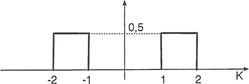
\includegraphics[scale=1]{graphique-Q-orale}
		\end{center}
		Soit $U = [0.15, 0.6, 0.53, 0.9, 0.34, 0.17, 0.82, 0.08, 0.507, 0.03]$ une séquence de 10 nombres aléatoires tirés à partir d'une distribution uniforme entre 0 et 1.\\
		L'étudiant devra~:
		\begin{itemize}
			\item estimer en utilisant la séquence $U$ par Monte Carlo la probabilité que $x(5) > 0.001$~;
			\item justifier de manière théorique (c.à-d. en utilisant les propriétés du système dynamique) le résultat du point précédent.
		\end{itemize}
		\pagebreak

		\subsection*{(Proposition de) réponse}
			Avant de partir plus loin il faut déjà qu'on comprenne le concept de "Monte Carlo".

			On à ici une liste $U$ de nombres aléatoires compris uniformément entre 0 et 1 et on nous demande de "transformer" ces nombres afin qu'ils soient distribués selon la fonction de densité ci-dessus.
			Vu l'allure de cette fonction, nos nombres "transformés" seront compris entre $[-2,-1] \cup [1, 2]$, puisque notre fonction de densité est une uniforme définie dans cet intervalle.\\

			Comme c'est une fonction de densité, on peux en calculer sa fonction de répartition (voir cours de Statistiques):
			\[
				F(x) = \int_{-\infty}^x f(t)\dif t =
				\begin{cases}
					0 &\text{ si } x < -2\\
					\frac{x+2}{2} &\text{ si } -2 \leq x \leq -1 \\
					\frac{1}{2} &\text{ si } -1 < x < 1 \\
					\frac{x}{2} &\text{ si } 1 \leq x \leq 2\\
					1 &\text{ si } x > 2.
				\end{cases}
			\]

			Graphique :

			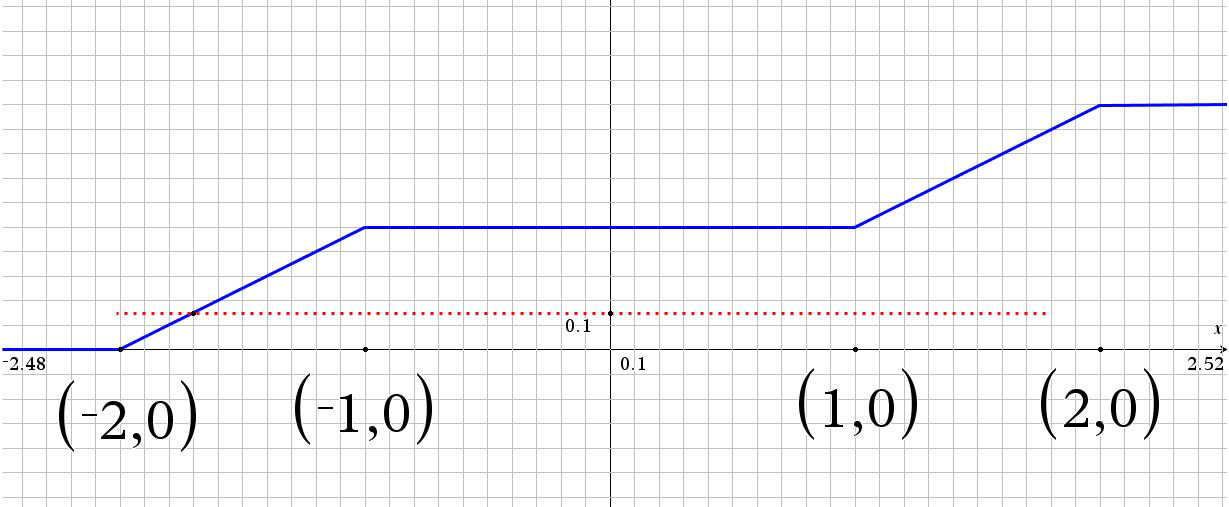
\includegraphics[width=\textwidth]{monte-carlo-fonction-distribution}

			La droite bleue représente le graphe de la fonction $F(x)$, la ligne rouge en pointillée est d'ordonnée la valeur du premier élément de $U$, à savoir $0.15$. \\

			Remarquons que les valeurs de $U$ sont toutes comprises entre 0 et 1, ce qui est également le cas de notre fonction de répartition (en ordonnée) (et le cas de toute fonction de répartition.
			Pour en déduire notre nouvelle liste $U'$ de nombre "transformés", il nous suffit donc de trouver le bon intervalle de la fonction de répartition, ce qui n'est en soit pas très compliqué car
			elle ne décroit jamais (à nouveau, comme toute fonction de répartition). \\

			Par exemple reprenons le premier point de $U$~: $0.15$, il se trouve dans le 2ème cas (i.e. $-2 \leq x \leq -1$, ici on le remarque facilement grâce au graphique. On doit maintenant calculer~:
			\[0.15 = \frac{x+2}{2} \Leftrightarrow x = -1.7,\]
			qui est bien compris dans les bornes de notre intervalle ($-2 \leq x \leq -1$), donc tout vas bien.

			À titre de contre-exemple, si on avait essayé avec le 4ème intervalle pour cette même valeur~: $0.15 = \frac{x}{2} \Leftrightarrow x = 0.3 $, qui n'est pas compris entre $1 \leq x \leq$.\\

			En pratique on est censé calculer la fonction réciproque (inverse) de $F(x)$, i.e. $F^{-1}(x)$ et du coup trouver les valeurs devient plus simple, mais ce n'est parfois pas évident de trouver analytiquement
			la réciproque. On appelle ça la \emph{méthode de la transformée inverse}.\\

			Une fois tous les points transformés un à un on obtient~:
			\[
				U' = [-1.7, 1.2, 1.06, 1.8, -1.32, -1.66, 1.64, -1.84, 1.014, -1.94]
			\]\\

			Reprenons notre système initiale:
			\begin{gather*}
					\dot{x} = K \cdot x\\
					\frac{\partial x}{\partial t} (t) = K \cdot x(t)\\
					x(t) = x(0) \cdot e^{K \cdot t}\\
					x(t) = 0.1 \cdot e^{K \cdot t}
			\end{gather*}
			On en déduit que $x(t=5) = 0.1 \cdot e^{5K} $. Il nous reste à calculer $P\left[x(5) > 0.001\right]$~:
			\begin{gather*}
					P\left[x(5) > 0.001\right]\\
					P\left[0.1 \cdot e^{5K} > 0.001\right]\\
					P\left[e^{5K} > 0.0001\right]\\
					P\left[K > -\frac{3}{5} \cdot \ln(10)\right] \approx P\left[K > -1.38\right]	\\
					F(-1.38) = 	\frac{-1.38 + 2}{2} \approx 0.31\\
					P\left[U > 0.31 \right] = 1-0.31 = 0.69 =69\%
			\end{gather*}
			Attention le U de la dernière ligne de calcul désigne la loi Uniforme sur $[0, 1]$ et non la liste $U$ de nombre donnée dans l'énoncé.\\

			Nous devrions donc avoir en toute logique dans notre liste $U, 69\%$ des éléments qui sont supérieur à $0.31$, dans notre cas nous en avons 6 sur les 10 éléments, soit $60\%$ ce qui n'est pas très loin du compte étant donné le petit jeu de données que nous avons.\\
			Si l'on reprends la liste $U'$ trouvés précédemment, on remarque qu'il y à également 6 éléments parmi les 10 qui sont supérieur à $-1.38$ (4ème ligne de calcul). Ce qui n'est pas une coïncidence.

\end{document}
